% Working manuscript, first drafted 2026-08-24; test results added 2026-10-02.
% IEEE version uses the IEEEtran conference format.
% Results are from the single preregistered G-12 test campaign (freeze
% g12freeze-f9608210..., results/g12/), exported by tools/export_g12_tables.py
% to presentation-results/data/g12_test_*.csv.
% Figures: python deliverables/research-paper/figures/make_figures.py
\documentclass[conference]{IEEEtran}

\usepackage{amsmath,amssymb}
\usepackage{booktabs}
\usepackage{graphicx}
\usepackage{microtype}
\usepackage[hidelinks]{hyperref}
\graphicspath{{figures/}}

\title{How Much of Deep Joint Source--Channel Coding's\\
Advantage Survives a Fair Comparison?\\
Evidence from Image Classification}

\author{
\IEEEauthorblockN{U. N. Kar, N. Ravi, S. Mukherjee, A. Mishra, T. Srivastava}
\IEEEauthorblockA{\textit{Vellore Institute of Technology, Andhra Pradesh, India}\\
nishchalravi05@gmail.com}
}

\begin{document}
\maketitle

\begin{abstract}
Deep joint source--channel coding (DJSCC) offers a different way to transmit images over bandwidth-constrained wireless channels. Instead of separately compressing an image and protecting the resulting bits against channel errors, DJSCC learns the source representation and its transmission jointly. For task-oriented applications, where the receiver may only need to classify an image rather than reconstruct it perfectly, this raises an important question: does the benefit come from joint source--channel coding itself, or simply from learning to transmit information that is more useful for the task?

This paper develops a controlled three-system framework for studying that question over a complex additive white Gaussian noise channel. The conventional digital system transmits JPEG~2000-compressed images using an NR-LDPC-based physical layer. A second, task-aware digital control uses the same transmission chain but replaces the conventional image representation with quantized learned features. The third system is an end-to-end DJSCC model that maps images directly to channel symbols and supports both reconstruction and classification at the receiver.

The three systems are given the same transmission budget and are tested under the same channel conditions and dataset splits. This lets us compare them more fairly and see whether any improvement comes from learning better features for classification, from learning how to transmit those features over the channel, or from both.

We evaluate all systems once, on the 3925 held-out Imagenette-160 test images at 21 SNRs from $-8$ to $18$~dB, after every model, operating point and analysis choice had been frozen on validation data. At a bandwidth ratio of $1/6$, averaged over three trained seeds, DJSCC classifies 76.1\% of images correctly at $-8$~dB, where neither digital system delivers any packets, and leads the adaptive JPEG~2000 system by 66 to 70 points from $-8$ to $-5$~dB. The two are statistically tied at $-4$ and $-3$~dB, and from $-2$~dB upward the JPEG~2000 system is more accurate, by about four points at high SNR (86.6\% against 82.4\% at 18~dB). The task-aware digital system reaches 81.1\% once its packets arrive; DJSCC exceeds it by 0.7 to 1.3 points from 1~dB upward, and the two are tied from $-4$ to 0~dB. All four preregistered hypotheses are supported. When the task-aware digital system uses a rate-1/5 code instead of rate~1/3, it delivers from $-7$~dB and scores 80.9\% from $-6$~dB, which leaves DJSCC a clear advantage only at $-7$~dB and below. The receiver's classifier matters as much as the link: scoring the same JPEG~2000 outputs with a classifier trained only on uncompressed images costs up to 43 points near the delivery threshold.


\begin{IEEEkeywords}
semantic communication, task-oriented communication, deep joint source--channel coding, image classification, 5G NR LDPC, JPEG 2000
\end{IEEEkeywords}
\end{abstract}

\section{Introduction}
Conventional communication systems usually treat source coding and channel coding as two separate problems. The source is first compressed into a digital bitstream. Redundancy is then added so that the bitstream can be protected against errors introduced by the channel. Shannon's separation theorem provides the classical foundation for this design: under its assumptions and with sufficiently long blocklengths, source and channel coding can be optimized independently without losing optimality~\cite{shannon1948,cover2006}.

Real systems do not operate in this asymptotic setting. They use finite blocklengths and must meet finite latency constraints. As a result, coding-rate back-off and nonzero decoding-failure probabilities matter in practice~\cite{polyanskiy2010,kostina2013}. Packetization and format overhead also consume part of the available transmission budget, leaving less room for the source payload itself.

This distinction becomes especially important when the receiver does not need a bit-perfect reconstruction of the original source. In machine-oriented communication, the real goal may be a downstream task such as classification, retrieval, or control. In that setting, transmitting every visual detail of an image may be unnecessary. A lower-dimensional representation can be sufficient if it preserves the information needed for the task. This motivates \emph{task-oriented}, or more broadly semantic, communication systems, where the transmitted representation is optimized for the receiver's objective rather than only for reconstruction quality.

Deep joint source--channel coding is one way to build such a system. Instead of first producing a compressed bitstream and then protecting it with a separate channel code, DJSCC uses a neural encoder to map the source directly to channel symbols. A differentiable channel model is placed between the transmitter and receiver during training, allowing the neural encoder and decoder to be optimized end to end~\cite{bourtsoulatze2019}. Early work on image transmission showed the well-known graceful-degradation behavior of neural JSCC~\cite{bourtsoulatze2019}. Later studies extended the idea to feedback, variable bandwidth, OFDM-oriented models, and transformer-based architectures~\cite{kurka2020feedback,kurka2021bandwidth,yang2021ofdm,yang2023witt}.

A simple learned-versus-digital comparison does not reveal why the learned system performs differently. A task-oriented DJSCC encoder changes two things at the same time. First, it can learn a representation that is tailored to the task. Second, it removes the usual boundary between source coding and channel coding. A conventional JPEG-based system changes neither of these: it sends a generic image representation and relies on a separate channel code for robustness.

This creates an attribution problem. If the learned system achieves higher task accuracy, the gain may come from the learned representation, from joint source--channel optimization, from limitations of the chosen digital baseline, or from some combination of these factors. For this reason, a controlled comparison needs a task-aware digital system in addition to the conventional reconstruction-oriented baseline.

There is also a second problem: the digital baseline must be given the same physical transmission budget as the learned system. Calling a baseline simply ``JPEG + LDPC'' is not enough, because finite-block overhead and the selected coding and modulation settings determine how much useful source data can actually be carried within a fixed number of complex channel uses. A digital baseline can also be unfairly weakened if it is forced to use a single operating point across every SNR.

To address both issues, the study is structured around three systems for task-oriented image classification. The first is a reconstruction-oriented separated baseline using JPEG 2000, a TS~38.212-derived 5G NR LDPC coding/rate-matching core, and BPSK, QPSK, or 16-QAM~\cite{jpeg2000,3gpp38212}. The second is a task-oriented separated digital control in which learned image features are quantized and sent through the same digital physical layer. The third is a task-aware DJSCC system that maps images directly to a fixed number of complex channel symbols and produces both reconstruction and classification outputs at the receiver. All design choices are made on the validation split, and all three systems are then evaluated once on the held-out test split.

The study therefore asks how much of DJSCC's advantage for classification survives when the digital baseline is given a fair chance. To our knowledge, it makes three contributions:
\begin{itemize}
\item a three-system comparison in which a reconstruction-oriented digital link and a task-aware digital link share one finite-block NR-LDPC chain, and the learned JSCC system uses the same complex-channel-use budget and $E_s/N_0$ convention;
\item a measurement of how strongly the receiver's classifier sets the outcome: scoring the same digital outputs with a classifier trained on uncompressed images instead of one fine-tuned on compressed images changes accuracy near the digital threshold by up to 43 points and widens the SNR range in which DJSCC leads by 3 to 9~dB;
\item an attribution of DJSCC's low-SNR advantage: at the main bandwidth ratio, learned task features sent over the same digital link come within 1.3 points of DJSCC on the test split, averaged over three seeds, wherever their packets arrive, and a lower-rate code moves their delivery threshold to $-7$~dB, so most of the advantage comes from avoiding outage rather than from a better task representation.
\end{itemize}
None of the three systems is new on its own. The contribution lies in the controls and in what they show about the comparison.

The experiments in this manuscript use image classification over a simulated complex AWGN channel. Top-1 classification accuracy is the primary task metric, while reconstruction quality is retained as a secondary diagnostic.

\section{Related Work}
\subsection{Deep JSCC and practical digital comparators}
DeepJSCC introduced end-to-end image transmission in which a neural encoder maps images directly to noisy-channel symbols instead of first producing a reliable intermediate bitstream~\cite{bourtsoulatze2019}. Later work extended the approach to feedback and bandwidth adaptation~\cite{kurka2020feedback,kurka2021bandwidth}. Constellation-constrained variants further showed that learned JSCC can operate with finite channel-input alphabets~\cite{tung2022}. Practical digital comparators have also appeared in earlier studies, where conventional image codecs were combined with finite-length LDPC coding and digital modulation rather than compared only through idealized channel-capacity limits~\cite{kurka2020feedback,tung2022}. Transformer-based JSCC has since been compared with BPG and 5G NR LDPC coding, with the modulation and code rate chosen separately at each SNR~\cite{yang2025swinjscc}, and other work argues that well-engineered separate source and channel coding remains competitive with JSCC~\cite{ren2025separate}. The present work therefore does not claim novelty for using a practical channel code or for comparing digital transmission with DeepJSCC.

\subsection{Task-oriented and digital semantic communication}
Task-oriented communication changes the receiver's objective from faithful reconstruction to a downstream inference task. For example, Jankowski \emph{et al.} compared learned digital feature transmission with direct learned feature-to-channel mappings for wireless image retrieval~\cite{jankowski2021}; their digital scheme assumed capacity-achieving channel codes. Information-bottleneck methods have been used to learn compact task-oriented features for edge inference~\cite{shao2022}, including a robust variant that encodes features into a discrete representation for digital modulation~\cite{xie2023}. Huang \emph{et al.} sent entropy-coded learned image features over a practical LDPC code, alongside BPG over the same code and DJSCC, for joint reconstruction and classification; the learned digital scheme led DJSCC wherever its bits decoded reliably and showed the digital cliff below that~\cite{huang2024}. Later work adapts the modulation order of such digital systems to the channel~\cite{park2025} and improves their vector quantizer~\cite{mao2026}. A task-aware digital arm is therefore not a new communication paradigm. In this study, its role is instead to act as an attribution control while sharing the same implemented digital physical layer as the reconstruction-oriented arm.

Using a learned JSCC receiver for both reconstruction and classification is also established in prior work. Lyu \emph{et al.} study semantic communication for simultaneous image recovery and classification~\cite{lyu2024}, while later work examines how reconstruction-oriented and task-oriented communication objectives can be aligned~\cite{diao2025}. Recent vector-quantized semantic systems have also compared conventional image coding, learned digital representations, and learned JSCC with practical channel coding~\cite{lokumarambage2026}. Accordingly, this paper does not claim the first three-family comparison or a novel dual-head architecture.

\subsection{Positioning of this study}
The contribution pursued here is mainly methodological. Unlike a simple learned-versus-digital comparison, the study controls both the transmitted representation and the choice between separated and joint source--channel coding. A reconstruction-oriented digital link and a task-oriented digital feature link share the same finite-block NR-LDPC/rate-matching chain, while the learned JSCC arm uses the same complex-channel-use budget and $E_s/N_0$ convention. This arrangement is intended to make differences between the three systems easier to attribute to the representation and coding strategy rather than to unequal transmission resources.

The study also controls the classifier at the receiver. Recognition models lose accuracy on compressed images mainly because they have not seen compression artifacts, and retraining them on compressed images recovers most of that loss~\cite{janeiro2023}. Learned-versus-digital comparisons nevertheless may classify the decoded digital images with a network trained on uncompressed images, as in~\cite{huang2024}. Here the digital outputs are scored by both a clean and an artifact-fine-tuned classifier, so the effect of that choice on the comparison can be measured.

\section{System Model and Problem Formulation}
\subsection{Source and channel-use budget}
Consider an image-label pair $(\mathbf{x},y)\sim\mathcal{D}$, where $\mathbf{x}\in[0,1]^{H\times W\times C}$ is an RGB image and $y\in\{1,\ldots,M\}$ is its class label. For Imagenette-160~\cite{imagenette}, $H=W=160$, $C=3$, and $M=10$. The source dimensionality is $n=HWC$. A communication system is allocated $k$ complex baseband channel uses per image, with bandwidth ratio
\begin{equation}
 r=\frac{k}{n}.
\end{equation}
The configured bandwidth-ratio set is
\begin{equation}
 r\in\left\{\frac12,\frac13,\frac16,\frac1{12},\frac1{24},\frac1{48}\right\}.
\end{equation}
For Imagenette-160, $n=76{,}800$, giving channel-use budgets of $38{,}400$, $25{,}600$, $12{,}800$, $6{,}400$, $3{,}200$, and $1{,}600$, respectively.

\begin{table}[t]
\caption{Imagenette-160 split sizes used in the study.}
\label{tab:datasets}
\centering
\begin{tabular}{lrrr}
\toprule
Dataset & Train & Val. & Test \\
\midrule
Imagenette-160 & 8469 & 1000 & 3925 \\
\bottomrule
\end{tabular}
\end{table}

\subsection{Channel model}
Let $\mathbf{z}\in\mathbb{C}^{k}$ denote the transmitter output before power normalization. The channel input is normalized independently per image as
\begin{equation}
 \tilde{\mathbf{z}}=\frac{\mathbf{z}}{\sqrt{\frac{1}{k}\sum_{i=1}^{k}|z_i|^2}},
\end{equation}
which imposes unit average symbol power. Transmission uses a memoryless complex AWGN channel,
\begin{equation}
 \mathbf{r}=\tilde{\mathbf{z}}+\gamma^{-1/2}\mathbf{n},
 \qquad \mathbf{n}\sim\mathcal{CN}(\mathbf{0},\mathbf{I}),
\end{equation}
where $\gamma=10^{\mathrm{SNR}_{\mathrm{dB}}/10}$. SNR is reported as $E_s/N_0$ per normalized complex channel use. For digital references stated in $E_b/N_0$,
\begin{equation}
 \left.\frac{E_s}{N_0}\right|_{\mathrm{dB}}=
 \left.\frac{E_b}{N_0}\right|_{\mathrm{dB}}+10\log_{10}(Q_mR_c),
\end{equation}
where $Q_m$ is coded bits per modulation symbol and $R_c$ is channel-code rate.

To make paired comparisons more controlled, the implementation uses a system-independent keyed noise identity. For a fixed image, SNR, seed, and channel-use budget, paired systems therefore receive the same deterministic AWGN realization whenever the representation permits such pairing.

\subsection{Task objective}
Each system ultimately produces class logits $\mathbf{s}\in\mathbb{R}^{M}$ and prediction $\hat y=\arg\max_j s_j$. The primary endpoint is top-1 task accuracy as a function of SNR,
\begin{equation}
 A(\gamma)=\Pr(\hat y=y\mid\gamma).
\end{equation}
PSNR and SSIM are retained as secondary reconstruction diagnostics, not substitutes for the downstream task endpoint.

\section{Compared Communication Systems}
\subsection{Reconstruction-oriented separated digital system}
The conventional arm is
\begin{equation}
\begin{split}
\mathbf{x} &\xrightarrow{\mathcal{C}_{\mathrm{J2K}}} \mathbf{b}_s
\xrightarrow{\mathcal{P}} \mathbf{b}_p
\xrightarrow{\mathcal{E}_{\mathrm{LDPC}}} \mathbf{b}_c
\xrightarrow{\mathcal{M}} \mathbf{z}\\
&\xrightarrow{\mathrm{AWGN}}\mathbf{r}
\xrightarrow{\mathcal{D}_{\mathrm{digital}}}\hat{\mathbf{x}}
\xrightarrow{h}\hat y.
\end{split}
\end{equation}
Here $\mathcal{C}_{\mathrm{J2K}}$ denotes JPEG 2000 source coding, $\mathcal{P}$ is our transport-block accounting and packetization logic, $\mathcal{E}_{\mathrm{LDPC}}$ is the TS~38.212-derived LDPC coding/rate-matching chain, and $\mathcal{M}$ represents BPSK, QPSK, or 16-QAM. Sionna 2.0.1~\cite{sionna} provides the LDPC encoder and decoder. Segmentation, CRC, filler handling, and transport accounting remain explicitly represented by the experiment.

For a chosen modulation, the coded-bit budget is $G=kQ_m$. The source payload is then chosen as the largest byte-aligned transport-block payload whose full coding and rate-matching representation fits inside $G$. Failed transmissions are not removed from evaluation. Structural infeasibility, codec infeasibility, decode failure, and successful delivery are recorded as distinct outcomes, and the prescribed outage outcome remains in the task-accuracy denominator.

\subsection{Task-aware learned JSCC system}
The learned joint system uses an encoder
\begin{equation}
 f_{\theta}:\mathbb{R}^{H\times W\times C}\rightarrow\mathbb{C}^{k},
\end{equation}
followed by the common power normalization and AWGN model. The encoder has two strided $5\times5$ convolutions with 64 and 128 channels, which downsample the image by a factor of four to a $40\times40$ grid, then two residual blocks with group normalization~\cite{wu2018gn} and PReLU activations~\cite{he2015prelu}. A final $3\times3$ convolution produces $2c$ real feature channels, and each pair becomes one complex symbol. The value of $c$ sets the bandwidth ratio: $c=8$ gives $1600\times8=12{,}800$ symbols at $r=1/6$, and $c=2$ gives $3200$ symbols at $r=1/24$.

The receiver has a reconstruction head and a classification head,
\begin{equation}
 g_{\phi}(\mathbf{r})=(\hat{\mathbf{x}},\mathbf{s}).
\end{equation}
Both heads share a decoder trunk that mirrors the encoder. The reconstruction head upsamples with two transposed convolutions. The classification head applies global average pooling to the 128-channel trunk output, followed by one linear layer. Training minimizes
\begin{equation}
 \mathcal{L}=\mathcal{L}_{\mathrm{CE}}(\mathbf{s},y)+\lambda\mathcal{L}_{\mathrm{MSE}}(\hat{\mathbf{x}},\mathbf{x}).
\end{equation}
The weight $\lambda$ was chosen from $\{0,0.1,0.3,1,3\}$ in a validation pilot at 7~dB, using a preregistered rule with a one-point accuracy tolerance and a PSNR floor on the reconstruction. The rule selected $\lambda=3$. The model has 1,567,197 parameters at $r=1/6$ and 1,539,537 at $r=1/24$.

\subsection{Task-oriented separated digital feature control}
The attribution control is
\begin{equation}
 \mathbf{x}\xrightarrow{q_{\psi}}\mathbf{u}
 \xrightarrow{\mathrm{quantize}}\mathbf{b}_u
 \xrightarrow{\mathrm{same\ digital\ link}}\hat{\mathbf{b}}_u
 \xrightarrow{d_{\omega}}\hat y.
\end{equation}
The feature encoder $q_{\psi}$ reuses the residual trunk of the DJSCC encoder. Its output is projected to a $D$-dimensional vector, and each element is quantized by a uniform 2-bit scalar quantizer. The quantized indices are range-coded with a static entropy model fitted on the training set. If range coding would produce more bits than the raw $2D$-bit representation, the raw form is sent instead, with a one-bit flag marking the choice. The message is then zero-padded to the transport-block payload and sent through the same CRC, LDPC, rate-matching, and modulation chain as the JPEG~2000 system, using the same $k$ channel uses. At the receiver, the decoded indices are dequantized and passed to a task head $d_{\omega}$.

The dimension $D$ was selected on validation data from $\{64,128,\ldots,2048\}$. Each candidate was trained and then evaluated through the real digital chain at 7~dB. Accuracy rose with $D$ from 28.4\% at $D=64$ to 82.0\% at $D=2048$, which was selected. With $D=2048$ the raw payload is 4096 bits. It fits a BPSK, rate-1/3 transport block at $r=1/6$, and that physical-layer setting is used at every SNR.

Rate~1/3 is the lowest LDPC rate in the search space of both digital systems, and it sets their delivery threshold. To see how far that threshold moves with a lower-rate code, a secondary variant sends a smaller task-aware model through a rate-1/5 code. It uses the $D=1024$ model from the same validation selection, unchanged, whose 2048-bit raw payload fits one BPSK transport block at rate~1/5 (base graph~2, 2544 payload bits) within the same $k$. This variant was added and validated before the test split was opened. It is reported descriptively and is not part of any hypothesis.

This system keeps task-aware representation learning but puts back a discrete boundary between source and channel coding. The three-way design therefore separates reconstruction-oriented digital transmission, task-aware digital transmission, and task-aware joint transmission. Comparing the first two measures the effect of changing the transmitted representation toward the task. Comparing the task-aware digital system with DJSCC measures what joint source--channel optimization adds on top of that. The feature encoders, quantization, and task heads differ between the two learned systems, so this second comparison is not a pure channel-coding contrast.

\subsection{Additional variants}
Table~\ref{tab:systems} lists every system variant evaluated. Besides the three main systems, the study includes:
\begin{itemize}
\item \emph{SNR-randomized DJSCC}, with the same architecture, trained with an SNR drawn per sample and per epoch from $\{1,4,7,13,19\}$~dB;
\item \emph{PAPR-capped DJSCC}, with the same architecture plus a projection after power normalization that limits the symbol-domain PAPR to 3~dB. The projection preserves each symbol's phase and finds, by bisection, a common scaling that keeps unit mean power while respecting the peak bound;
\item a \emph{reconstruction ablation}, in which the DJSCC reconstruction $\hat{\mathbf{x}}$ is classified by the clean-trained ResNet-18 instead of the DJSCC task head;
\item two restricted JPEG~2000 baselines: one fixed to QPSK with the rate and resolution still adapted, and one fixed to a single operating point (16-QAM, LDPC rate 1/2, full resolution) at every SNR;
\item a \emph{baseline JPEG} system, which replaces JPEG~2000 with baseline JPEG and is selected in the same way;
\item a \emph{label transmission} system, in which the transmitter runs the task-aware digital model to completion and sends only its predicted label, a 4-bit field in a one-byte frame, as the first byte of the same packet used by the task-aware digital system;
\item the \emph{rate-1/5 task-aware digital} variant described above.
\end{itemize}

\begin{table}[t]
\caption{System variants evaluated on the test split. Every variant uses the same complex AWGN channel and the same $k$ for its bandwidth ratio. Seeds: number of trained (or, for the untrained digital codecs, channel) seed pairs evaluated.}
\label{tab:systems}
\centering
\footnotesize
\begin{tabular}{@{}p{0.40\columnwidth}ccp{0.27\columnwidth}@{}}
\toprule
Variant & $r$ & Seeds & Classifier at receiver \\
\midrule
DJSCC (7~dB training) & $1/6$ & 3 & Own task head \\
 & $1/24$ & 1 & Own task head \\
DJSCC, SNR-randomized & $1/6$ & 1 & Own task head \\
DJSCC, PAPR-capped & $1/6$ & 1 & Own task head \\
DJSCC reconstruction & $1/6$ & 1 & Clean ResNet-18 \\
JPEG~2000 + LDPC, adaptive & $1/6$ & 3 & Fine-tuned ResNet-18 \\
 & $1/24$ & 1 & Fine-tuned ResNet-18 \\
JPEG~2000 + LDPC, QPSK only & $1/6$ & 1 & Fine-tuned ResNet-18 \\
JPEG~2000 + LDPC, fixed MCS & $1/6$ & 3 & Fine-tuned ResNet-18 \\
Baseline JPEG + LDPC & $1/6$ & 1 & Fine-tuned ResNet-18 \\
Task-aware digital & $1/6$ & 3 & Own task head \\
Task-aware digital, rate 1/5 & $1/6$ & 1 & Own task head \\
Label transmission & $1/6$ & 1 & Transmitter's prediction \\
\bottomrule
\end{tabular}
\end{table}

\subsection{Receiver classifiers}
Two ResNet-18 classifiers~\cite{he2016resnet} read images at the receiver. The clean classifier is trained from scratch on the uncompressed Imagenette training images. The fine-tuned classifier starts from the clean one and is trained for a further 20 epochs on 44,039 JPEG~2000-decoded versions of the training images. The compression settings are drawn from the operating points the baseline can select at or below 7~dB. The fine-tuned classifier is the primary scorer for every JPEG~2000 and JPEG variant, because a classifier that has never seen compression artifacts would understate what the digital system delivers. Scores from the clean classifier on the same received images are also kept and are reported in Section~\ref{sec:scorer}.

\section{Experimental Protocol}
\label{sec:protocol}
\subsection{Datasets and split discipline}
Imagenette-160 is used for the experiments, with 8469 training, 1000 validation, and 3925 test images across 10 classes. Dataset membership and sample identities are fixed through versioned manifests. The published training partition is deterministically divided into project training and validation subsets, while the published Imagenette validation partition is used as the project test split.

Every model, checkpoint, operating point, classifier, analysis rule and hypothesis window was chosen on the training and validation data and then recorded in a freeze manifest, which was committed to the project repository before the test loader would open. The test split was then evaluated once, in a single campaign that ran every variant in Table~\ref{tab:systems}. Section~\ref{sec:repro} records two execution faults in that campaign and how they were handled; neither changed a measurement.

\subsection{Training}
All learned models are trained from scratch with Adam~\cite{kingma2015adam} at a learning rate of $10^{-3}$, cosine decay to zero without warm-up, batch size 32, 100 epochs, and mixed-precision arithmetic. Augmentation is a random resized crop and a horizontal flip. Unless stated otherwise, the channel SNR during training is fixed at 7~dB, and the checkpoint with the highest validation accuracy at 7~dB is kept. Final DJSCC models were trained for three paired training and channel seeds at each bandwidth ratio, and the task-aware digital model for three seeds at $r=1/6$. The SNR-randomized and PAPR-capped variants were trained once each. On the test split, the three main systems and the fixed-MCS baseline at $r=1/6$ are evaluated in all three seed pairs; the digital codecs have no trained seed, so for them the three pairs differ only in the channel noise. Every other variant is evaluated in the first seed pair.

\subsection{Digital operating-point selection}
For each SNR and bandwidth ratio, the JPEG~2000 system selects an encoding resolution (a downsampled image size, upsampled bicubically at the receiver), an LDPC rate from $\{1/3,1/2,2/3,5/6\}$, and a modulation from BPSK, QPSK, and 16-QAM. The JPEG~2000 codestream is the largest one that fits in the transport-block payload. Selection maximizes the expected number of correct classifications on the validation split,
\begin{equation}
 \mathbb{E}[A]=P_{\mathrm{s}}\,A_{\mathrm{codec}}+(1-P_{\mathrm{s}})\,A_{\mathrm{out}},
\end{equation}
where $P_{\mathrm{s}}$ is the probability that every code block decodes, taken from the measured BLER curves; $A_{\mathrm{codec}}$ is the measured validation accuracy of the fine-tuned classifier on error-free decoded images at that setting; and $A_{\mathrm{out}}$ is the measured accuracy of the outage rule. Exact ties are broken in favor of the more reliable link, then the lower-order modulation, the lower code rate, and the larger image. The outage rule predicts a fixed class (class~0) whenever a packet fails or no feasible encoding exists. On the class-balanced validation split this rule scores exactly 10.0\%, and every failed transmission stays in the accuracy denominator.

The selection is analytic, but the reported accuracy is not: every selected operating point is re-run image by image through the full chain, and the realized outcome is what is reported. The learned models are trained once and are not adapted to the test SNR. This asymmetry favors the digital baseline, and it is intentional.

\subsection{Paired evaluation and hypotheses}
Each system is evaluated on the same 3925 test images at 21 SNRs: $-8$ to $7$~dB in 1~dB steps, then 9, 11, 13, 15, and 18~dB. The AWGN realization for each image depends only on the image identity, the SNR, the channel seed, and $k$, so systems at the same bandwidth ratio see the same noise wherever their representations allow it.

The statistical target is the paired, image-level difference in top-1 accuracy between two systems at a fixed SNR and bandwidth ratio. Each image's outcome is first averaged over the three seed pairs, and the stable image identity is the resampling unit, so every interval is paired across systems and SNRs within each resample. All intervals use one shared set of 10,000 image bootstrap resamples and are two-sided 95\% percentile intervals unless stated otherwise. Four hypotheses, their decision rules, and their thresholds were fixed before the test split was opened:
\begin{itemize}
\item \emph{H1 (low-SNR separation).} DJSCC against the adaptive JPEG~2000 system at $r=1/6$. An SNR point qualifies when the studentized paired mean difference exceeds 1.96. H1 is supported if the longest run of consecutive qualified points at or below the 7~dB training SNR has at least three points and a calibrated p-value for that run is at most 0.05. The calibration resamples a Rademacher multiplier on each image's centred trajectory 10,000 times and recomputes the longest run. The mean paired difference over the whole region at or below 7~dB is reported as the effect size.
\item \emph{H2 (graceful versus cliff).} DJSCC against the fixed-MCS JPEG~2000 system over the 4~dB window in which that system lost the most accuracy on validation data, which is 3 to 7~dB. H2 is supported if the one-sided 95\% lower bound on the digital system's drop across the window is at least 30 points and the one-sided 95\% upper bound on DJSCC's drop is at most 15 points.
\item \emph{H3 (convergence).} DJSCC against the adaptive JPEG~2000 system at $r=1/6$. H3 is supported if, each as a one-sided 95\% bound, the weighted least-squares slope of the paired gap against SNR is negative, the gap at $-8$~dB is positive, and the gap at $18$~dB is smaller in magnitude than the gap at $-8$~dB.
\item \emph{H4 (attribution).} The H1 rule, with the task-aware digital system in place of the JPEG~2000 system. Joint coding is credited only to the extent that DJSCC also exceeds this control.
\end{itemize}
The remaining variants are reported descriptively. A design study on validation data, run before the final models were trained, estimated that at 80\% power the smallest paired difference H4 could detect at a single point is 1.8 to 1.9 points above the digital cliff and about 4 points below it.

Bandwidth-ratio selection for the classical system is based on validation data rather than on learned-versus-classical test results. This keeps the choice of operating point separate from the comparison it is later used to evaluate. The ratio $1/6$ was selected as the main comparison ratio and $1/24$ as the low-bandwidth ratio.

\section{Implementation Checks}
\subsection{Reference classifier and learned-model profile}
The clean ResNet-18 reaches 898/1000 on the validation split after 100 epochs, above the target of 0.88. It has 11,181,642 parameters.

At $r=1/2$ the DJSCC model has 1,640,957 parameters. A batch-32 profile on an RTX 4060 Laptop GPU measured 1.004~GiB of peak reserved memory and 48.7~s per epoch, or about 1.35~h for 100 epochs.

\subsection{LDPC conformance and BLER characterization}
The TS~38.212-derived LDPC core was checked against an independent reference implementation with $K=128$, $N=256$, base graph 2, lifting size 22, rate $1/2$, offset min-sum decoding, and 5000 blocks per SNR point. Across BPSK, QPSK, and 16-QAM, the waterfall at BLER $10^{-2}$ is within 0.0037~dB of the reference. Packetization was checked across 216 configurations, of which 215 are feasible and one is structurally infeasible under the configured budget.

The BLER curves used for selection cover 3213 physical-layer operating points in 153 curves, at 5000 trials each (16,065,000 block trials in total). Operating points without a measured curve are excluded from selection rather than assigned a default BLER.

\subsection{Classical validation sweep}
The classical validation sweep evaluated 288 structural configurations over all 1000 validation images, for 288,000 image--configuration evaluations. Of these, 264,000 were delivered and 24,000 were codec-infeasible, with no decode or structural failures. Selection produced a valid operating point for all 378 requested SNR cells.

\begin{table}[t]
\caption{Implementation checks.}
\label{tab:validation}
\centering
\begin{tabular}{@{}p{0.27\columnwidth}p{0.67\columnwidth}@{}}
\toprule
Item & Result \\
\midrule
Clean classifier & 0.898 validation top-1 (898/1000), ResNet-18 trained from scratch \\
DJSCC profile & 1,640,957 parameters at $r=1/2$; 1.004 GiB peak reserved VRAM at batch 32 \\
LDPC conformance & Waterfall offset $\leq0.0037$ dB at BLER $10^{-2}$ against the reference decoder \\
BLER campaign & 153 curves; 3213 points; 5000 trials/point; 16,065,000 trials total \\
\bottomrule
\end{tabular}
\end{table}

\section{Test Results}
All results in this section are on the 3925 test images. Entries for the main systems are averaged over three seed pairs; the others come from the first seed pair. Table~\ref{tab:results} gives the accuracy of every variant at selected SNRs, Table~\ref{tab:hyp} the four preregistered tests, and Fig.~\ref{fig:differences} the paired differences behind them. A 95\% interval on a single accuracy here is about $\pm1.1$ points.

\begin{table*}[t]
\caption{Test top-1 accuracy (\%) at selected SNRs, 3925 images per entry. Rows marked ``3 seeds'' are averaged over three seed pairs; all others are the first seed pair, and ``seed 0'' gives DJSCC for that pair alone. Entries of 9.9 are the outage rule applied to every image (the share of the fixed fallback class in the test split). The digital systems use the operating point selected on validation data for each SNR; the learned models are trained once.}
\label{tab:results}
\centering
\begin{tabular}{llrrrrrrrrr}
\toprule
& & \multicolumn{9}{c}{SNR $E_s/N_0$ (dB)} \\
\cmidrule(l){3-11}
$r$ & System & $-8$ & $-6$ & $-4$ & $-2$ & $0$ & $4$ & $7$ & $9$ & $18$ \\
\midrule
$1/6$ & DJSCC (3 seeds) & 76.1 & 79.1 & 80.8 & 81.4 & 81.6 & 82.1 & 82.3 & 82.3 & 82.4 \\
 & \quad seed 0 & 71.5 & 76.3 & 79.3 & 80.5 & 81.1 & 81.5 & 82.0 & 82.0 & 82.1 \\
 & DJSCC, SNR-randomized & 77.6 & 80.0 & 81.1 & 82.1 & 82.6 & 82.9 & 82.6 & 82.8 & 83.0 \\
 & DJSCC, PAPR-capped & 76.7 & 79.3 & 81.0 & 81.4 & 81.8 & 82.4 & 82.3 & 82.0 & 82.3 \\
 & DJSCC reconstruction, clean classifier & 44.1 & 52.5 & 60.3 & 65.3 & 70.9 & 75.8 & 77.3 & 77.4 & 78.0 \\
 & JPEG~2000 + LDPC, adaptive (3 seeds) & 9.9 & 9.9 & 81.6 & 83.2 & 85.9 & 86.2 & 86.5 & 84.3 & 86.6 \\
 & \quad same outputs, clean classifier & 9.9 & 9.9 & 59.2 & 78.2 & 84.4 & 86.4 & 87.5 & 85.2 & 87.6 \\
 & JPEG~2000 + LDPC, QPSK only & 9.9 & 9.9 & 9.9 & 9.9 & 85.9 & 86.2 & 86.5 & 86.5 & 86.5 \\
 & JPEG~2000 + LDPC, fixed MCS (3 seeds) & 9.9 & 9.9 & 9.9 & 9.9 & 9.9 & 9.9 & 86.5 & 86.5 & 86.5 \\
 & Baseline JPEG + LDPC & 9.9 & 9.9 & 66.4 & 74.5 & 81.2 & 85.1 & 85.5 & 9.9 & 86.1 \\
 & Task-aware digital (3 seeds) & 9.9 & 9.9 & 81.1 & 81.1 & 81.1 & 81.1 & 81.1 & 81.1 & 81.1 \\
 & Task-aware digital, rate 1/5 & 9.9 & 80.9 & 80.9 & 80.9 & 80.9 & 80.9 & 80.9 & 80.9 & 80.9 \\
 & Label transmission & 9.9 & 9.9 & 81.0 & 81.0 & 81.0 & 81.0 & 81.0 & 81.0 & 81.0 \\
\midrule
$1/24$ & DJSCC & 47.3 & 59.1 & 68.3 & 73.9 & 76.3 & 78.8 & 79.8 & 80.0 & 80.0 \\
 & JPEG~2000 + LDPC, adaptive & 9.9 & 9.9 & 9.9 & 28.9 & 68.0 & 81.6 & 84.9 & 81.5 & 86.3 \\
 & \quad same outputs, clean classifier & 9.9 & 9.9 & 9.9 & 13.5 & 25.2 & 59.2 & 79.8 & 80.0 & 85.9 \\
\bottomrule
\end{tabular}
\end{table*}

\begin{table}[t]
\caption{Preregistered hypotheses on the test split, $r=1/6$, three seed pairs. Differences are DJSCC minus the comparator, in points; intervals are 95\%.}
\label{tab:hyp}
\centering
\footnotesize
\setlength{\tabcolsep}{3pt}
\begin{tabular}{@{}lp{0.55\columnwidth}c@{}}
\toprule
& Result & Decision \\
\midrule
H1 & Qualified run $-8$ to $-5$~dB (4 points), calibrated $p=0.030$; mean difference at or below 7~dB 14.6 [13.7, 15.4] & Supported \\
H2 & Fixed-MCS drop 3$\to$7~dB 76.7 (lower bound 75.5); DJSCC drop 0.2 (upper bound 0.4); difference 76.5 [75.1, 77.9] & Supported \\
H3 & Gap slope $-1.71$ points/dB [$-1.76$, $-1.67$]; gap $+66.3$ at $-8$~dB, $-4.2$ at 18~dB & Supported \\
H4 & Longest qualified run 1 to 7~dB (7 points), also $-8$ to $-5$~dB; calibrated $p=0.0096$; mean difference at or below 7~dB 17.6 [17.0, 18.2] & Supported \\
\bottomrule
\end{tabular}
\end{table}

\subsection{DJSCC and the adaptive JPEG~2000 baseline}
Fig.~\ref{fig:headline} shows the main comparison at $r=1/6$. DJSCC produces a usable prediction at every SNR, with no delivery failures by construction. Averaged over three seeds, its accuracy falls from 82.4\% at 18~dB to 76.1\% [75.0, 77.2] at $-8$~dB, a loss of about six points across the 26~dB range.

The JPEG~2000 system delivers nothing from $-8$ to $-5$~dB and scores the outage floor of 9.9\%. At $-4$~dB every packet decodes and accuracy jumps to 81.6\%. The paired differences (Fig.~\ref{fig:differences}) separate three regions. From $-8$ to $-5$~dB DJSCC leads by 66.3 to 70.2 points, and these four points form the qualified run that supports H1. At $-4$ and $-3$~dB the two are tied: DJSCC is 0.9 and 0.7 points behind, with intervals that include zero. From $-2$~dB upward the JPEG~2000 system is ahead at every SNR, by 1.8 points at $-2$~dB and by 3.8 to 4.3 points from $-1$~dB upward, apart from 9~dB, where the gap is 2.0 points because 3.1\% of digital packets fail. The measured transition lies between $-5$ and $-4$~dB; no SNR between those two points was evaluated.

The paired gap shrinks steadily as SNR rises, by 1.71 points per dB [1.67, 1.76], from $+66.3$ points at $-8$~dB to $-4.2$ points at 18~dB, which supports H3. The convergence ends in a crossing rather than a tie: at high SNR the digital system is about four points more accurate.

Table~\ref{tab:oppoints} lists the operating points the baseline uses, as selected on validation data. Just above the transition it sends a $64\times64$ image with BPSK and a rate-1/3 code, the most robust setting available, in a 531-byte payload of which 157 bytes are JPEG~2000 headers. It moves to larger images and higher-order modulation as the channel improves; at 11~dB and above, the 4262-byte payload spends 3.7\% on headers. Two operating points deliver less than every packet on the test split, as they did on validation: 2.3\% of packets fail at $-2$~dB and 3.1\% at 9~dB. At 9~dB the selected setting sits on the steep part of its BLER curve, where the analytic prediction used for selection and the image-by-image run differ by a few percent of packets.

\begin{figure}[t]
\centering
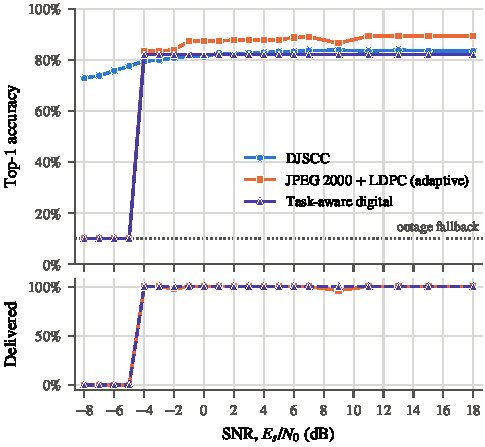
\includegraphics[width=\columnwidth]{fig_headline}
\caption{Test accuracy (top) and fraction of packets delivered (bottom) at $r=1/6$. DJSCC, JPEG~2000 + LDPC and the task-aware digital system are averaged over three seed pairs, with shaded 95\% intervals; the rate-1/5 task-aware variant is one seed pair. DJSCC is scored by its own task head, JPEG~2000 by the ResNet-18 fine-tuned on JPEG~2000 artifacts. The dotted line is the outage rule. Lines join measured points only.}
\label{fig:headline}
\end{figure}

\begin{figure}[t]
\centering
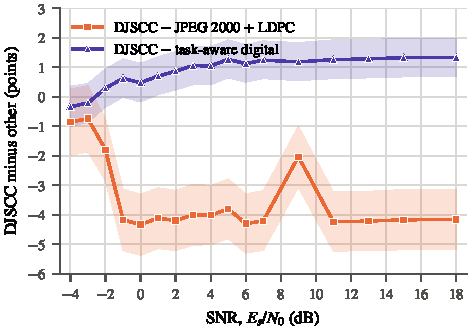
\includegraphics[width=\columnwidth]{fig_differences}
\caption{Paired difference in test accuracy, DJSCC minus each digital system, at $r=1/6$, averaged over three seed pairs, with 95\% image-bootstrap intervals. Below $-4$~dB both digital systems deliver nothing and DJSCC leads both by 66 to 70 points (not shown).}
\label{fig:differences}
\end{figure}

\begin{table}[t]
\caption{Operating points of the adaptive JPEG~2000 baseline at $r=1/6$, selected on validation data, with test accuracy and delivered fraction (three seed pairs).}
\label{tab:oppoints}
\centering
\footnotesize
\setlength{\tabcolsep}{4pt}
\begin{tabular}{@{}lcccrr@{}}
\toprule
SNR (dB) & Image & LDPC & Mod. & Acc. (\%) & Deliv. (\%) \\
\midrule
$-8$ to $-5$ & 160 & 1/3 & BPSK & 9.9 & 0.0 \\
$-4$, $-3$ & 64 & 1/3 & BPSK & 81.6 & 100.0 \\
$-2$ & 96 & 1/2 & BPSK & 83.2 & 97.7 \\
$-1$, $0$ & 128 & 1/3 & QPSK & 85.9 & 100.0 \\
$1$ & 128 & 2/3 & BPSK & 85.9 & 100.0 \\
$2$ to $5$ & 128 & 1/2 & QPSK & 86.2 & 100.0 \\
$6$ & 160 & 5/6 & QPSK & 86.5 & 100.0 \\
$7$ & 160 & 1/2 & 16-QAM & 86.5 & 100.0 \\
$9$ & 160 & 2/3 & 16-QAM & 84.3 & 96.9 \\
$11$ to $18$ & 160 & 2/3 & 16-QAM & 86.6 & 100.0 \\
\bottomrule
\end{tabular}
\end{table}

\subsection{Graceful degradation against a fixed digital link}
H2 compares DJSCC with the JPEG~2000 system fixed to a single operating point (16-QAM, rate 1/2, full resolution) over the 3 to 7~dB window, which was chosen on validation data as the window in which that system loses the most accuracy. On the test split, the fixed system loses 76.7 points across the window (86.5\% at 7~dB, 9.9\% at 3~dB), with a one-sided lower bound of 75.5 against the 30-point threshold. DJSCC loses 0.2 points, with an upper bound of 0.4 against the 15-point threshold. H2 is supported. The comparison describes the cliff of a non-adaptive link; the adaptive baseline has no comparable cliff above $-4$~dB because it changes its operating point.

\subsection{Bandwidth ratio}
Fig.~\ref{fig:bandwidth} repeats the comparison at $r=1/24$, with 3200 channel uses per image (first seed pair). DJSCC loses most at low SNR: at $-8$~dB it falls from 71.5\% to 47.3\% against the same seed pair at $r=1/6$, while at 18~dB it drops only from 82.1\% to 80.0\%. The JPEG~2000 system delivers nothing up to $-3$~dB. At $-2$~dB it delivers 82.0\% of packets, but the images that arrive are heavily compressed and it classifies only 28.9\% of all test images correctly. DJSCC stays ahead up to $+1$~dB, by 4.9 to 8.4 points from $-1$ to $+1$~dB, and the JPEG~2000 system is ahead from $+2$~dB, by 0.6 to 6.3 points. Reducing the channel uses fourfold therefore moves the first SNR at which the digital system is ahead from $-2$~dB to $+2$~dB. These are single-seed differences; at $+2$ and $+3$~dB they are within the spread expected between seeds.

\begin{figure*}[t]
\centering
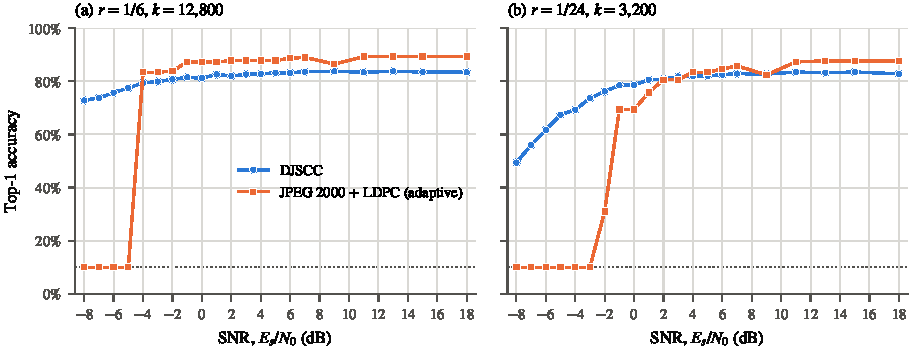
\includegraphics[width=\textwidth]{fig_bandwidth}
\caption{DJSCC against the adaptive JPEG~2000 baseline on the test split at two bandwidth ratios. (a) Three seed pairs with 95\% intervals; (b) the first seed pair. Reducing the channel uses fourfold moves the first SNR at which the digital system is ahead from $-2$~dB to $+2$~dB. Scorers and selection as in Fig.~\ref{fig:headline}.}
\label{fig:bandwidth}
\end{figure*}

\subsection{Task-aware digital control}
\label{sec:er9}
The task-aware digital system (Fig.~\ref{fig:headline}) behaves like the JPEG~2000 system on the delivery axis. It fails completely up to $-5$~dB and delivers every packet from $-4$~dB. Once its packets arrive, its accuracy is constant at 81.1\% (81.0\%, 81.2\%, and 81.1\% in the three seed pairs), because error-free delivery reproduces the transmitter's quantized features exactly.

Against DJSCC (Fig.~\ref{fig:differences}), the two are tied from $-4$ to 0~dB, with paired differences between $-0.3$ and $+0.6$ points whose intervals include zero. From 1~dB upward DJSCC is ahead at every SNR, by 0.7 to 1.3 points, and these seven consecutive points from 1 to 7~dB form the longest qualified run that supports H4. Below $-4$~dB DJSCC leads by the same 66 to 70 points as against the JPEG~2000 system, which is the second qualified run. Joint source--channel coding is therefore credited with two things at this ratio: avoiding the outage below $-4$~dB, and a residual of about one point once both systems deliver. The second is real on the test split but small, and smaller than the four-point lead of the JPEG~2000 system over DJSCC in the same range. The features and the task heads of the two learned systems differ, so the residual is not a pure channel-coding effect.

Against the JPEG~2000 system, the delivered features score 81.1\% and the delivered images 81.6\% to 86.6\%. That difference cannot be attributed to the representation: the features are read by a single linear layer, the images by a fine-tuned ResNet-18 with about seven times as many parameters as the whole DJSCC model.

The label transmission system scores 81.0\% wherever it delivers, identical to the task-aware digital system in the same seed pair, because it sends that system's own prediction. It also fails below $-4$~dB. That is a property of the implementation: the one-byte label is carried in the task-aware system's 4096-bit packet, so it inherits that packet's decoding threshold. This variant therefore bounds the accuracy of transmitting a decision, not the SNR at which a decision can be transmitted.

\subsection{Effect of the code-rate floor}
Both digital systems are limited by the same design choice: no code rate below 1/3. The rate-1/5 task-aware variant (Fig.~\ref{fig:headline}) removes that limit for the feature link. It delivers 66.4\% of packets at $-7$~dB, scoring 56.9\%, and every packet from $-6$~dB, scoring 80.9\%. At $-6$ and $-5$~dB it is 1.8 and 0.9 points more accurate than the three-seed DJSCC average, at $-4$ and $-3$~dB the two are level, and above that it is within 1.5 points of DJSCC. Its accuracy once delivered is 0.2 points below the rate-1/3 system, because it sends 1024 instead of 2048 features. With a lower-rate code, the SNR range in which DJSCC is clearly the only working system shrinks from $-5$~dB and below to $-7$~dB and below. This variant is one seed pair and is not part of any hypothesis; it shows how much of the low-SNR comparison is set by the digital code-rate floor.

\subsection{Effect of the receiver classifier}
\label{sec:scorer}
Fig.~\ref{fig:scorer}(a) scores the same JPEG~2000 outputs with both classifiers. From 2~dB upward the two agree within about one point, and the clean classifier is the slightly better one at high SNR (87.6\% against 86.6\% at 18~dB). Just above the delivery transition they do not agree: at $-4$~dB the fine-tuned classifier scores 81.6\% and the clean one 59.2\%. With the clean classifier, DJSCC would lead the JPEG~2000 system up to $-2$~dB instead of being tied at $-4$~dB. At $r=1/24$ the difference is larger, 68.0\% against 25.2\% at 0~dB, and with the clean classifier DJSCC would lead or tie up to 9~dB instead of $+1$~dB. Near the cliff the baseline sends small, heavily compressed images, and a classifier trained on such images is worth up to 43 points, consistent with the finding that retraining on compressed images recovers most of a recognition model's loss~\cite{janeiro2023}. The crossover SNR reported for this kind of comparison therefore depends on the classifier at the receiver as well as on the transmission scheme.

Fig.~\ref{fig:scorer}(b) holds the DJSCC transmission fixed and changes the receiver. Classifying the DJSCC reconstruction with the clean ResNet-18 scores 44.1\% at $-8$~dB and 78.0\% at 18~dB, well below the jointly trained task head at every SNR. The reconstruction is trained with $\lambda=3$ and is blurred at low SNR. The task head reads the decoder features directly and does not depend on image quality in the same way.

\begin{figure*}[t]
\centering
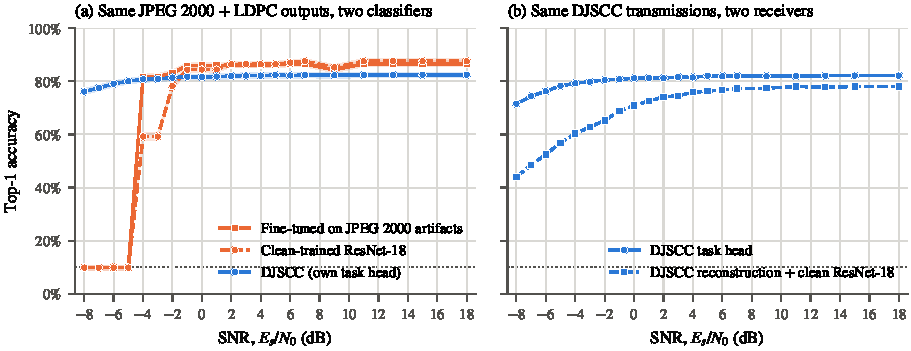
\includegraphics[width=\textwidth]{fig_scorer}
\caption{(a) The same JPEG~2000 + LDPC outputs at $r=1/6$ scored by the fine-tuned and the clean ResNet-18, with DJSCC for reference (three seed pairs). (b) The same DJSCC transmissions read by the DJSCC task head and by the clean ResNet-18 applied to the DJSCC reconstruction (first seed pair).}
\label{fig:scorer}
\end{figure*}

\subsection{Training variants: SNR randomization and peak power}
Fig.~\ref{fig:training} compares the three DJSCC models at $r=1/6$ in the first seed pair, the only pair in which the two variants were trained. Training at randomized SNRs gives 77.6\% against 71.5\% at $-8$~dB, and the PAPR-capped model 76.7\%. That difference is not evidence for either training change: the other two seed pairs of the fixed-SNR model score 78.4\% and 78.5\% at $-8$~dB, so the spread between seeds of one training recipe is as large as the difference between recipes. Above 0~dB all three models are within 1.5 points.

Over the test images the fixed-SNR DJSCC encoder has a mean symbol-domain PAPR of 13.3 to 14.8~dB across seed pairs and a maximum of 24.7~dB. For comparison, the adaptive JPEG~2000 system at 18~dB, which uses 16-QAM, has a mean of 2.6~dB and a maximum of 3.3~dB. The PAPR-capped model has a maximum of 3.000002~dB, within the 3~dB cap and its $10^{-4}$~dB numerical tolerance, at an accuracy within about one point of the fixed-SNR model above 0~dB. PAPR here is measured on the complex symbols, not on an oversampled, pulse-shaped waveform, so it does not establish the peak power of a transmitted RF signal.

\begin{figure}[t]
\centering
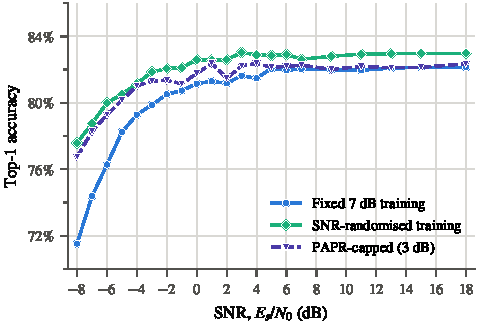
\includegraphics[width=\columnwidth]{fig_training}
\caption{DJSCC at $r=1/6$ on the test split, first seed pair: trained at a fixed 7~dB, trained with SNR drawn from $\{1,4,7,13,19\}$~dB, and trained with a 3~dB symbol PAPR cap. The other two seed pairs of the fixed-SNR model score 78.4\% and 78.5\% at $-8$~dB. Note the vertical scale.}
\label{fig:training}
\end{figure}

\subsection{Restricted digital baselines}
Fig.~\ref{fig:controls} shows what the adaptivity of the baseline is worth. Restricting the modulation to QPSK delays the first delivery from $-4$ to $-1$~dB, with the same plateau of 86.5\%. The single fixed operating point (16-QAM, rate 1/2) delivers nothing below 7~dB and reaches 86.5\% above it, a drop of 76.6 points between 7 and 6~dB. A baseline with a single operating point would have made DJSCC look far better than the adaptive baseline does.

Replacing JPEG~2000 with baseline JPEG costs up to 15.2 points just above the transition (66.4\% against 81.6\% at $-4$~dB), with smaller differences at higher SNR. This is consistent with JPEG's larger header overhead, which takes a large share of a small payload. The fine-tuned classifier was trained on JPEG~2000 artifacts, not JPEG artifacts, which also counts against the JPEG curve. At 9~dB the JPEG operating point selected on validation data failed on every test image, as it did on validation; that setting delivers every packet at 11~dB, so the 9~dB point lies on the steep part of its BLER curve. The measurement is reported as observed.

\begin{figure}[t]
\centering
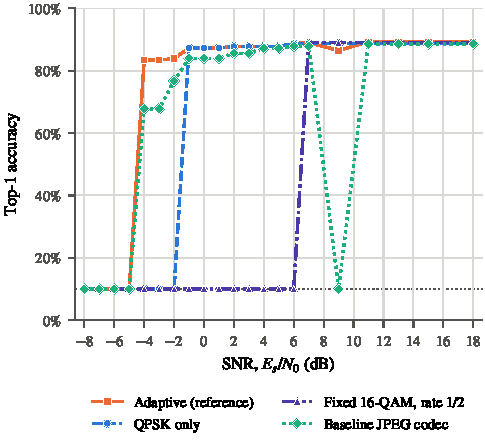
\includegraphics[width=\columnwidth]{fig_controls}
\caption{Adaptive JPEG~2000 + LDPC at $r=1/6$ on the test split against restricted versions: QPSK only (rate and resolution still adapted), one fixed operating point at all SNRs, and baseline JPEG in place of JPEG~2000. All scored by the fine-tuned ResNet-18.}
\label{fig:controls}
\end{figure}

\subsection{Reproducibility of the test campaign}
\label{sec:repro}
The freeze manifest, the per-image outcomes of every test unit (their digests are listed in a committed manifest), the result tables, and the analysis output are archived with the project code. Two execution faults occurred during the single test campaign, and both are recorded there. The first launch stopped before any model produced an output on a test image, because a record-keeping guard still refused test-split records; the guard was corrected, the freeze was re-issued for the corrected code, and the campaign was started again. Later, the label-transmission system stopped on a self-check that compared its output with a fingerprint of its validation run, which cannot match on different images; the check was restricted to validation data, and a descriptive McNemar p-value in the analysis was changed from floating-point to exact integer arithmetic after it overflowed at the test-set size. Each change is recorded with the exact files and contents it altered. None of them changed a model, an operating point, a noise draw, an analysis rule, or any reported accuracy, and no outcome was selected, repeated, or discarded.

\section{Discussion}
The test results support the qualitative picture that motivated the study, but only over a narrow range. DJSCC degrades gradually and the separated systems have a cliff, and all four preregistered hypotheses hold. At $r=1/6$, however, the cliff lies between $-5$ and $-4$~dB. At $-4$ and $-3$~dB the adaptive digital baseline is level with DJSCC, and from $-2$~dB upward it is more accurate by about four points. At this ratio DJSCC wins where the digital system delivers nothing. At $r=1/24$ DJSCC also wins up to $+1$~dB, where the digital packets arrive but carry too few bytes for the classifier to do well on the decoded image.

Much of the high-SNR gap reflects a difference in accuracy ceilings. DJSCC with its jointly trained head saturates near 82\%, and the task-aware digital system near 81\%. The fine-tuned ResNet-18 on well-delivered JPEG~2000 images reaches 86.6\%, and the clean one 87.6\%. The DJSCC task head is a single linear layer on pooled decoder features. A deeper head, or a stronger backbone of the kind used in recent transformer-based JSCC work~\cite{yang2023witt}, might narrow this gap. We did not test that, and the parameter count of the learned model was deliberately kept well below that of the reference classifier.

The task-aware digital control changes the attribution question. It reaches 81.1\% whenever its packets decode, within 1.3 points of DJSCC, and below the cliff it fails in the same way as the JPEG~2000 system. H4 shows that joint coding adds something beyond outage avoidance at this operating point, about one point once both systems deliver, but most of what DJSCC gains at low SNR comes from avoiding outage, not from a better task representation. The rate-1/5 variant makes the same point from the other side: with a lower-rate code, the same kind of digital feature link works down to $-7$~dB and is ahead of DJSCC at $-6$ and $-5$~dB.

The comparison also shows how sensitive such conclusions are to the baseline. Holding the transmission fixed, the choice of receiver classifier moves the crossover by about 3~dB at $r=1/6$ and about 9~dB at $r=1/24$. Removing adaptivity moves it by 9~dB, from $-2$ to 7~dB. Replacing the codec with JPEG lowers the digital curve by up to 15 points, and lowering the digital code-rate floor from 1/3 to 1/5 moves the digital threshold by 2 to 3~dB. Each of these choices, made the other way, would have made DJSCC look better. We made the baseline as strong as the preregistered search space allowed. At $r=1/6$ the learned system then wins only where the baseline cannot deliver; at $r=1/24$ it also wins where the baseline delivers too few bytes for the classifier to do well.

\section{Limitations}
The three main systems at $r=1/6$ are evaluated over three seed pairs; every other variant is one seed pair. Between seed pairs DJSCC varies by up to seven points at $-8$~dB and by under one point above 0~dB, so single-seed differences of a few points at low SNR, including those between the training variants, are not interpreted. For the digital codecs the three seed pairs differ only in the channel noise and are nearly identical.

The digital operating points, checkpoints, the task-aware feature dimension, and $\lambda$ were chosen on the 1000 validation images. The test split was not used for any choice, but the search space itself was fixed in advance, and the lowest code rate in it, 1/3, sets the delivery threshold of both digital systems. The rate-1/5 variant indicates how much that matters for the feature link; a rate-1/5 JPEG~2000 baseline was not evaluated.

The learned and digital systems are scored by different classifiers. The headline comparison is therefore a whole-system comparison and not a comparison of channel codes. Section~\ref{sec:scorer} reports both scorers for the digital outputs so that the effect can be seen.

The channel is simulated complex AWGN with perfect synchronization and known SNR at the receiver. Fading, carrier and timing offsets, and hardware nonlinearity are not modeled, and PAPR is measured in the symbol domain only. The systems are compared at equal channel uses and equal average symbol energy; this is a statement about accuracy at equal resources, not a measured energy saving. Computational cost at the transmitter and receiver is not compared. The dataset is a 10-class subset of ImageNet at $160\times160$ pixels, and the results are not shown to transfer to larger label sets or other image sizes.

\section{Conclusion}
We built a controlled comparison of three ways to send an image to a remote classifier: JPEG~2000 over a 5G NR LDPC link with per-SNR adaptation, learned task features over the same link, and task-aware DJSCC, all with the same number of complex channel uses, and evaluated them once on a held-out test split under preregistered rules. On Imagenette-160 at $r=1/6$, DJSCC is the only system that works at or below $-5$~dB, where it keeps 76\% to 80\% accuracy averaged over three seeds. It is level with the adaptive digital baseline at $-4$ and $-3$~dB, and from $-2$~dB upward the baseline is more accurate by about four points. At $r=1/24$ the DJSCC advantage extends to $+1$~dB. The task-aware digital control is within 1.3 points of DJSCC wherever it delivers, and with a rate-1/5 code it delivers from $-7$~dB. Avoiding the outage cliff therefore accounts for most of DJSCC's low-SNR gain, and how far that gain extends depends on the digital system's lowest code rate and on the classifier at the receiver.

Two extensions follow directly. A label-transmission link sized for its 4-bit payload would show how far a transmitted decision, rather than a representation, can reach. Hardware experiments with a software-defined radio, which would measure real waveforms and impairments, would test whether the ordering found on a simulated AWGN channel survives a real one.

\section*{Acknowledgment}
The research idea and direction of this project are the authors' own, and Sections~I--III and the first two paragraphs of the abstract were written by the authors. Generative AI tools were used as follows. Anthropic's Claude Opus~5.5 produced initial drafts of Sections~IV--X and the results paragraph of the abstract, generated Figs.~1--6 from the project's published result tables, made minor edits and citation additions in Sections~I and~II, checked all references against publisher records, and produced the supplementary material (pseudo-code, code excerpts, and tables generated from the published result files). Claude Opus~5.5 and OpenAI's GPT-5.6 Sol assisted in writing the simulation, training, and analysis code whose methods and results are described in Sections~IV--VII. All code, results, figures, text, and references were reviewed and verified by the authors, who take full responsibility for the content of this paper and its supplementary material.

\begin{thebibliography}{30}
\bibitem{shannon1948} C. E. Shannon, ``A mathematical theory of communication,'' \emph{Bell System Technical Journal}, vol. 27, no. 3, pp. 379--423, and no. 4, pp. 623--656, 1948.
\bibitem{cover2006} T. M. Cover and J. A. Thomas, \emph{Elements of Information Theory}, 2nd ed. Hoboken, NJ, USA: Wiley, 2006.
\bibitem{polyanskiy2010} Y. Polyanskiy, H. V. Poor, and S. Verd\'u, ``Channel coding rate in the finite blocklength regime,'' \emph{IEEE Transactions on Information Theory}, vol. 56, no. 5, pp. 2307--2359, 2010.
\bibitem{kostina2013} V. Kostina and S. Verd\'u, ``Lossy joint source--channel coding in the finite blocklength regime,'' \emph{IEEE Transactions on Information Theory}, vol. 59, no. 5, pp. 2545--2575, 2013.
\bibitem{bourtsoulatze2019} E. Bourtsoulatze, D. B. Kurka, and D. G\"und\"uz, ``Deep joint source--channel coding for wireless image transmission,'' \emph{IEEE Transactions on Cognitive Communications and Networking}, vol. 5, no. 3, pp. 567--579, 2019.
\bibitem{kurka2020feedback} D. B. Kurka and D. G\"und\"uz, ``DeepJSCC-f: Deep joint source--channel coding of images with feedback,'' \emph{IEEE Journal on Selected Areas in Information Theory}, vol. 1, no. 1, pp. 178--193, 2020.
\bibitem{kurka2021bandwidth} D. B. Kurka and D. G\"und\"uz, ``Bandwidth-agile image transmission with deep joint source--channel coding,'' \emph{IEEE Transactions on Wireless Communications}, vol. 20, no. 12, pp. 8081--8095, 2021.
\bibitem{yang2021ofdm} M. Yang, C. Bian, and H.-S. Kim, ``Deep joint source channel coding for wireless image transmission with OFDM,'' in \emph{Proc. IEEE ICC}, 2021, pp. 1--6.
\bibitem{yang2023witt} K. Yang, S. Wang, J. Dai, K. Tan, K. Niu, and P. Zhang, ``WITT: A wireless image transmission transformer for semantic communications,'' in \emph{Proc. IEEE ICASSP}, 2023, pp. 1--5.
\bibitem{jpeg2000} ISO/IEC 15444-1:2019 $|$ ITU-T T.800, ``Information technology---JPEG 2000 image coding system: Core coding system,'' 2019.
\bibitem{3gpp38212} 3GPP, ``NR; Multiplexing and channel coding,'' 3GPP TS 38.212, V17.13.0 (Release 17), Feb. 2026.
\bibitem{tung2022} T.-Y. Tung, D. B. Kurka, M. Jankowski, and D. G\"und\"uz, ``DeepJSCC-Q: Constellation constrained deep joint source--channel coding,'' \emph{IEEE Journal on Selected Areas in Information Theory}, vol. 3, no. 4, pp. 720--731, 2022.
\bibitem{yang2025swinjscc} K. Yang, S. Wang, J. Dai, X. Qin, K. Niu, and P. Zhang, ``SwinJSCC: Taming Swin transformer for deep joint source--channel coding,'' \emph{IEEE Transactions on Cognitive Communications and Networking}, vol. 11, no. 1, pp. 90--104, 2025.
\bibitem{ren2025separate} T. Ren, R. Li, M.-M. Zhao, X. Chen, G. Liu, Y. Yang, Z. Zhao, and H. Zhang, ``Separate source channel coding is still what you need: An LLM-based rethinking,'' \emph{ZTE Communications}, vol. 23, no. 1, pp. 30--44, 2025.
\bibitem{jankowski2021} M. Jankowski, D. G\"und\"uz, and K. Mikolajczyk, ``Wireless image retrieval at the edge,'' \emph{IEEE Journal on Selected Areas in Communications}, vol. 39, no. 1, pp. 89--100, 2021.
\bibitem{shao2022} J. Shao, Y. Mao, and J. Zhang, ``Learning task-oriented communication for edge inference: An information bottleneck approach,'' \emph{IEEE Journal on Selected Areas in Communications}, vol. 40, no. 1, pp. 197--211, 2022.
\bibitem{xie2023} S. Xie, S. Ma, M. Ding, Y. Shi, M. Tang, and Y. Wu, ``Robust information bottleneck for task-oriented communication with digital modulation,'' \emph{IEEE Journal on Selected Areas in Communications}, vol. 41, no. 8, pp. 2577--2591, 2023.
\bibitem{huang2024} J. Huang, D. Li, C. Huang, X. Qin, and W. Zhang, ``Joint task and data-oriented semantic communications: A deep separate source--channel coding scheme,'' \emph{IEEE Internet of Things Journal}, vol. 11, no. 2, pp. 2255--2272, 2024.
\bibitem{park2025} J. Park, Y. Oh, S. Kim, and Y.-S. Jeon, ``Joint source--channel coding for channel-adaptive digital semantic communications,'' \emph{IEEE Transactions on Cognitive Communications and Networking}, vol. 11, no. 1, pp. 75--89, 2025.
\bibitem{mao2026} X. Mao, Q. Yan, B. Dai, X. Tang, and Z. Zhou, ``On the effectiveness of task-oriented digital semantic communication system,'' \emph{IEEE Transactions on Cognitive Communications and Networking}, vol. 12, pp. 3436--3451, 2026.
\bibitem{lyu2024} Z. Lyu, G. Zhu, J. Xu, B. Ai, and S. Cui, ``Semantic communications for image recovery and classification via deep joint source and channel coding,'' \emph{IEEE Transactions on Wireless Communications}, vol. 23, no. 8, pp. 8388--8404, 2024.
\bibitem{diao2025} Y. Diao, Y. Zhang, C. She, P. G. Zhao, and E. L. Li, ``Aligning task- and reconstruction-oriented communications for edge intelligence,'' \emph{IEEE Journal on Selected Areas in Communications}, vol. 43, no. 7, pp. 2575--2588, 2025.
\bibitem{lokumarambage2026} M. Lokumarambage, T. Sivalingam, H. Rezaei, N. Rajatheva, and A. Fernando, ``Edge computing-based vector quantized semantic communication system for wireless image transmission,'' \emph{IEEE Transactions on Consumer Electronics}, vol. 72, no. 3, pp. 5661--5670, 2026.
\bibitem{janeiro2023} J. M. Janeiro, S. Frolov, A. El-Nouby, and J. Verbeek, ``Are visual recognition models robust to image compression?'' arXiv:2304.04518, 2023.
\bibitem{imagenette} J. Howard, ``Imagenette,'' GitHub repository, 2019. [Online]. Available: \url{https://github.com/fastai/imagenette}
\bibitem{sionna} J. Hoydis \emph{et al.}, ``Sionna: An open-source library for next-generation physical layer research,'' arXiv:2203.11854, 2022.
\bibitem{wu2018gn} Y. Wu and K. He, ``Group normalization,'' in \emph{Proc. ECCV}, 2018, pp. 3--19.
\bibitem{he2015prelu} K. He, X. Zhang, S. Ren, and J. Sun, ``Delving deep into rectifiers: Surpassing human-level performance on ImageNet classification,'' in \emph{Proc. IEEE ICCV}, 2015, pp. 1026--1034.
\bibitem{he2016resnet} K. He, X. Zhang, S. Ren, and J. Sun, ``Deep residual learning for image recognition,'' in \emph{Proc. IEEE CVPR}, 2016, pp. 770--778.
\bibitem{kingma2015adam} D. P. Kingma and J. Ba, ``Adam: A method for stochastic optimization,'' in \emph{Proc. ICLR}, 2015.
\end{thebibliography}

\end{document}
